\documentclass[preprint, 3p,
authoryear]{elsarticle} %review=doublespace preprint=single 5p=2 column
%%% Begin My package additions %%%%%%%%%%%%%%%%%%%

\usepackage[hyphens]{url}

  \journal{An awesome journal} % Sets Journal name

\usepackage{graphicx}
%%%%%%%%%%%%%%%% end my additions to header

\usepackage[T1]{fontenc}
\usepackage{lmodern}
\usepackage{amssymb,amsmath}
% TODO: Currently lineno needs to be loaded after amsmath because of conflict
% https://github.com/latex-lineno/lineno/issues/5
\usepackage{lineno} % add
\usepackage{ifxetex,ifluatex}
\usepackage{fixltx2e} % provides \textsubscript
% use upquote if available, for straight quotes in verbatim environments
\IfFileExists{upquote.sty}{\usepackage{upquote}}{}
\ifnum 0\ifxetex 1\fi\ifluatex 1\fi=0 % if pdftex
  \usepackage[utf8]{inputenc}
\else % if luatex or xelatex
  \usepackage{fontspec}
  \ifxetex
    \usepackage{xltxtra,xunicode}
  \fi
  \defaultfontfeatures{Mapping=tex-text,Scale=MatchLowercase}
  \newcommand{\euro}{€}
\fi
% use microtype if available
\IfFileExists{microtype.sty}{\usepackage{microtype}}{}
\usepackage[]{natbib}
\bibliographystyle{plainnat}

\ifxetex
  \usepackage[setpagesize=false, % page size defined by xetex
              unicode=false, % unicode breaks when used with xetex
              xetex]{hyperref}
\else
  \usepackage[unicode=true]{hyperref}
\fi
\hypersetup{breaklinks=true,
            bookmarks=true,
            pdfauthor={},
            pdftitle={Morphometric Variations in Nepalese Bamboo: Investigating Diameter-Length Relationships in Two Major Groups},
            colorlinks=false,
            urlcolor=blue,
            linkcolor=magenta,
            pdfborder={0 0 0}}

\setcounter{secnumdepth}{5}
% Pandoc toggle for numbering sections (defaults to be off)


% tightlist command for lists without linebreak
\providecommand{\tightlist}{%
  \setlength{\itemsep}{0pt}\setlength{\parskip}{0pt}}







\begin{document}


\begin{frontmatter}

  \title{Morphometric Variations in Nepalese Bamboo: Investigating
Diameter-Length Relationships in Two Major Groups}
    \author[Institute of Forestry]{Sushila Sapkota%
  %
  \fnref{1}}
   \ead{sapkotasushila2001@gmail.com} 
    \author[Ministry of Forest and Environment]{Prakash Lamichhane%
  \corref{cor1}%
  \fnref{2}}
   \ead{forester.prakash@gmail.com} 
    \author[Institute of Forestry]{Sandeep Mahara%
  %
  \fnref{1}}
   \ead{maharas450@gmail.com} 
    \author[Forest Research and Training Center, Nepal]{Ananda Khadka%
  %
  \fnref{3}}
   \ead{anandakhadka@gmail.com} 
    \author[Institute of Forestry]{Suman Bhattarai%
  %
  \fnref{1}}
   \ead{sumancha004@gmail.com} 
      \affiliation[Institute of Forestry]{
    organization={Tribhuwan University},addressline={Pokhara - 15,
Hariyokharka,
Kaski},city={Pokhara,},postcode={33700},state={Gandaki},country={Nepal},}
    \affiliation[Ministry of Forest and Environment]{
    organization={Ministry of Forest and
Environment},addressline={Kathmandu-11, Singha
Durbar},city={Kathmandu,},postcode={44600},country={Nepal},}
    \affiliation[Forest Research and Training Center]{
    organization={Ministry of Forest and
Environment},addressline={Kathmandu-11, Singha
Durbar},city={Kathmandu,},postcode={44600},country={Nepal},}
    \cortext[cor1]{Corresponding author}
    \fntext[1]{This is the first author footnote.}
    \fntext[2]{Another author footnote.}
  
  \begin{abstract}
  Bamboo belongs to the Poaceae (Gramineae) family of grasses and is
  well known for its ecological services as well as engineering
  services. Quanntifying the dimensions of the bamboo shoot is crucial
  for further valuation of each of the service it provides. It is
  difficult to measure, especially the length of the bamboo, as length
  is a complex dimension of the bamboo plant. There were no prior
  research records depicting the correlation of diameter and height
  variables in Nepal.The research provides the measurment of the height
  (length) of the bamboo for its quantification in terms of biomass as
  well as its carbon content. We examined the relationship between the
  diameter and length of the Bambusa group and the Dendrocalamus group
  found in Nepal. Field data was taken from 650 sample plots (circular
  plots with a 56.42m radius) established by the Forest Research and
  Training Center (FRTC), covering 66 districts of Nepal. A multiple
  linear regression model was developed where 80\% of the data was
  considered as training data and the rest as testing data. The length
  served as an independent variable, whereas diameter at breast height
  (dbh), base, and height up to culmination were used as independent
  variables. We used the Shapiro Wilk test to check the normality of the
  dataset, and the classical Levene's test to test the variance of the
  data sets used for predictions. The regression coefficients were
  tested using a Welch's two-sample t-test. From the results, the best
  fitting equation for the Bambusa group was 0.907 * ht\_culmination +
  0.248 * dbh + 0.8078 * base + 0.141, and for the Dendrocalamus group
  was 0.978 * ht\_culmination + (-0.025) * dbh + 0.505 * base + 1.745.
  The best results were obtained when all three variables were used as
  independent, i.e., dbh, base, and height of culmination. The study
  opens up the space for further research focused on volume calculation
  of culms, biomass estimation, etc.
  \end{abstract}
    \begin{keyword}
    Bamboo \sep Biometrics \sep Linear Regression \sep 
    Diameter- Height Relationship
  \end{keyword}
  
 \end{frontmatter}

\hypertarget{introduction}{%
\section{Introduction:}\label{introduction}}

Bamboo belongs to the Poaceae (Gramineae) family of grasses (Tamang et
al., 2013) and is well known for providing ecological services, such as
erosion control, riverbank protection, landslide prevention, land
rehabilitation, soil moisture retention, biodiversity preservation, and
carbon sequestration (Bhattacharya et al., 2009). Due to its economic
value and varied applications in human living, it is referred to as
``green gold'' (Yeasmin et al., 2015). As the plant with the quickest
rate of growth on earth, with a growth range of 30-100cm per day in a
growing season (Zakikhani et al., 2017), it is commonly classified as a
woody plant because of its woody vascular bundle structure. In general,
they grow in a wide range of climates, from tropical to temperate
regions (Li \& Kobayashi 2004, Meena et al.~2019). There exist
approximately 1,250 distinct species distributed across 75 genera within
the global bamboo taxonomic classification (Tamang et al., 2013). It is
ubiquitously dispersed within tropical and subtropical regions spanning
approximately 46°N to 47°S, encompassing a collective expanse of
approximately 31.5 million hectares (FAO, 2005). This constituted
approximately 0.8\% of the global forested area as of the year 2010
(Song et al., 2011). The predominant distribution of bamboo occurs in
Asia, specifically within tropical and subtropical regions, with
significant concentrations in China (626 species), India (102 species),
Japan (84 species), Myanmar (75 species), and Malaysia (50 species),
where the cumulative bamboo-covered area in these regions is estimated
to exceed 1.8×10\^{}7 hectares, as reported by Shanmughavel and Francis
(1996), Singh and Singh (1999), Embaye et al.~(2003), Gratani et
al.~(2008), and Yen et al.~(2010). In contrast, Africa displays the
lowest bamboo species richness, totaling only five species (Das et al.,
2005). However, Nepal on the other hand, records a total of 13 bamboo
species (Bista et al., 2022).

Statistical analysis involving regression, as explained by Belsley et
al.~(2005), is employed to scrutinize the association between a
dependent variable (referred to as the result or response variable) and
one or more independent variables (termed predictors or explanatory
variables). The development of reliable tools supporting informed
decision-making in sustainable forestry necessitates accurate
predictions of both existing resource levels and anticipated resource
changes resulting from the implementation of specific management
alternatives, as highlighted by Tenzin and Hasenauer (2017). The
application of regression models facilitates the identification of
trends and patterns, prediction of future occurrences, and exploration
of the impact of one or more independent variables on the dependent
variable. To achieve precise estimations of forest biomass and carbon
storage at both regional and global scales, a comprehensive
comprehension of the Height-Diameter (H-D) relationship is imperative.
This is particularly significant given that numerous large-scale studies
rely on allometric equations that integrate the Height-Diameter
relationship (Feldpausch et al., 2011; Gao et al., 2016).

Although bamboo has many advantages and there is increasing demand for
its products in the country, there is little published information on
bamboo that demonstrates the relationship between its morphological
characteristics (Oli, 2005; Bista et al., 2022). Thus, the models
developed from the research will be important operational tools for
supporting decision-making for a wide range of activities in the studied
area. They have the capacity to depict the transient growth of trees
(diameter, height, and volume), provide intricate insights into the
evolution of stand structure (diameter and height distribution), compute
projections for biomass and carbon stock, and facilitate the inspection
of a multitude of silvicultural interventions and directives, among
other functionalities (Briseno et al., 2020). Thus, this study will be a
pioneering work for new researchers to develop the appropriate growth
model for diverse valuable species. The model employed in this study
presupposes a linear association between the dependent variable and the
independent variables, representing a specific category within the realm
of regression models.

\hypertarget{methodology}{%
\section{Methodology:}\label{methodology}}

\hypertarget{study-area}{%
\subsection{Study Area}\label{study-area}}

For the study, the bamboo potential area found in the non-forest area of
Nepal has been chosen. The seven bamboo species of Nepal majorly include
the two genera, i.e., Bambusa and Dendrocalamus. A total of 66 districts
of Nepal from east to west (28.3949 ◦ N, 84.124 ◦ E) were included in
the study area, chosen and finalized by Forest Research and Training
Center (FRTC).

\begin{figure}

{\centering 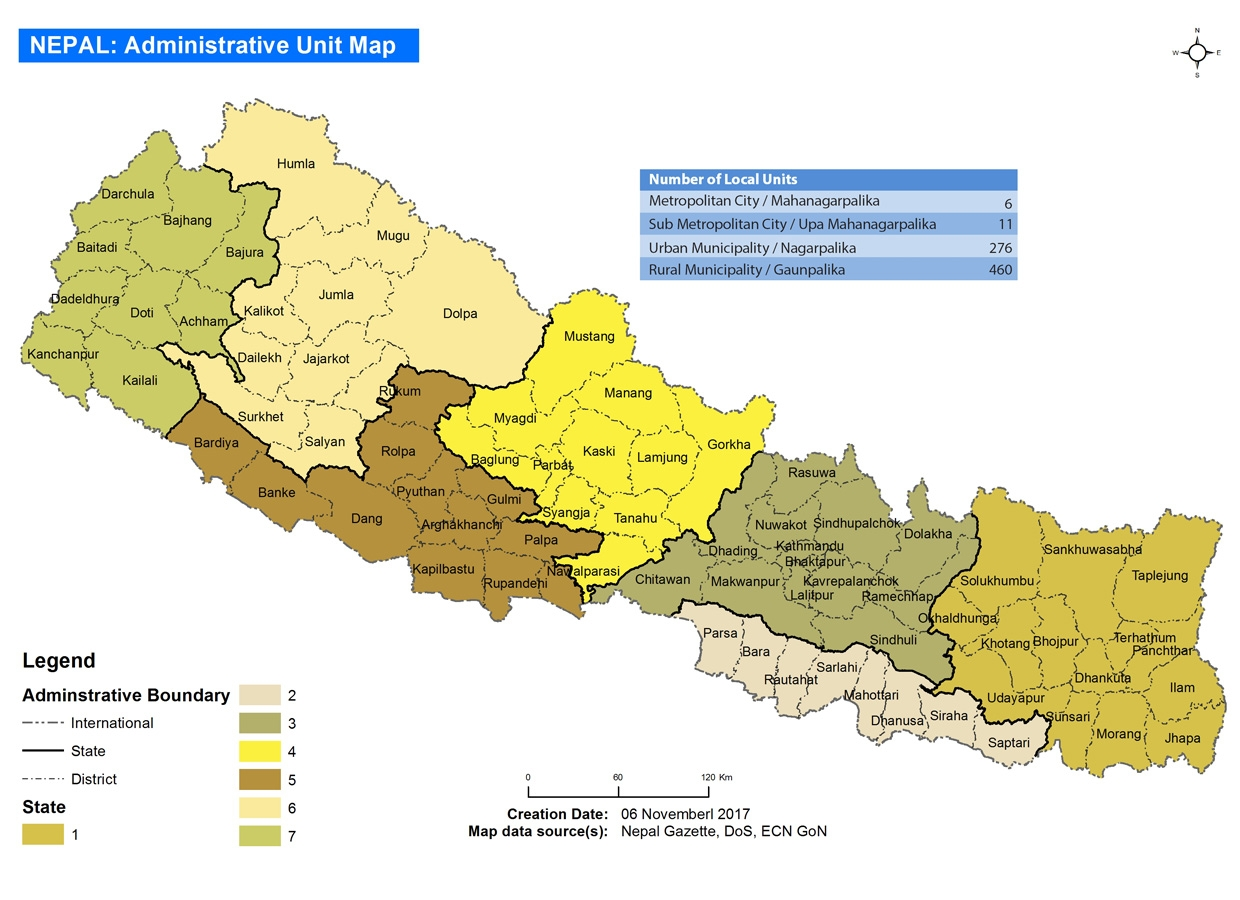
\includegraphics{../nepal} 

}

\caption{Study Area Map}\label{fig:unnamed-chunk-1}
\end{figure}

\hypertarget{sampling-method}{%
\subsection{Sampling Method}\label{sampling-method}}

The data for this assessment were collected from the inventory of 800
sample plots over Nepal, of which 650 plots were chosen with Normalized
Difference vegetation Index (NDVI) greater than 0.4, 150 plots had an
NDVI less than 0.4, and the rest 50 were non-bamboo plots selected by
visual interpretation by systematic point sampling (every fifth).
However, only the plots with NDVI greater than 0.4 were used for data
analysis, as it was assumed that NDVI values below 0.4 were not
represented by the annual green stand of bamboo and were confirmed later
by field verification too. The input points for visual interpretation
have been generated from the entire area of interest using a 1 x 1 km
grid in the entire country. Plots were chosen with the help of the
connect earth online (CEO) app. Inventory was done through circular
plots with a radius of 56.42m. The diameter at breast height (dbh), and
the diameter above 30cm from the (ground) base (d30) was measured.
Height i.e., up to the point of culmination (vertical) was measured with
the help of a vertex; total height was calculated with the help of the
Pythagoras theorem. For that, the base distance was also calculated from
the seedling point of bamboo in the field. A total of nine culms (three
culms from each size class) were measured from each clump based on size
class. The size class was defined as:

\begin{enumerate}
\def\labelenumi{\alph{enumi}.}
\item
  Less than 4.5 cm as Small
\item
  4.5cm to 7.5cm as Medium
\item
  More than 7.5cm as Large
\end{enumerate}

Rest was counted only according to age class, mainly defined as:

\begin{enumerate}
\def\labelenumi{\alph{enumi}.}
\item
  Less than 1 year
\item
  1-2 years
\item
  More then 3 years
\end{enumerate}

Identification of age class and species was done on the basis of
presence or absence of a sheath, the color of the culm, and with the
help of local resource person (LRP).

Figure 2: Bamboo Height Measurement

Here in Figure 2, `H' stands for the height culmination of the bamboo,
i.e., the height from the ground to the point where the bamboo starts to
lean. It was calculated with the help of a vertex. `b' stands for the
base distance from the seedling point of bamboo, and `tc' stands for the
height of bamboo, which was calculated by using the Pythagoras theorem
as a square root of (square of tc + square of base(b)) as almost of the
bamboos are leaning. Lastly, `l' stands for the total length of the
bamboo, which was measured after the felling of the bamboo. Since the
data used here was collected from destructive sampling, the bamboo culm
to be felled was previously inventoried. d30, dbh, height up to
culmination, and base were read orderly. Then the culm was finally
felled. After felling, stump height, number of nodes, and diameter at
different sections were measured. Also, the total length of the culm was
measured up to the tip with the help of a linear tape. The data from 369
individual culms was taken for the study.

\hypertarget{data-collection}{%
\subsection{Data collection}\label{data-collection}}

\hypertarget{primary-data-collection}{%
\subsubsection{Primary Data Collection}\label{primary-data-collection}}

The main aim for this study was to assess and update bamboo resources
information in Nepal in order to identify, map their distribution,
collect samples, estimate volume, biomass, and growing stock of bamboo
resources outside the forest area. Information on sample plots, methods
adopted during sampling, and sample plot measurement were done according
to the FRTC protocols, National Bamboo Resource Inventory Nepal (NBRAN)
(proposed), and strictly following instructions from FRTC officials.
Data were noted on the field tally sheets specially prepared for the
Bamboo Resource Inventory by FRTC.

\hypertarget{secondary-data-collection}{%
\subsubsection{Secondary Data
Collection}\label{secondary-data-collection}}

Other secondary data were gathered through a comprehensive review of
various manuals, published reports, and literature prepared by the FRTC,
particularly about bamboo, and several other published reports and
articles from different sources on the internet were taken into
consideration during the whole data analysis.

\hypertarget{data-analysis}{%
\subsection{Data analysis}\label{data-analysis}}

The analysis of the data involved the utilization of diverse software;
QGIS, statistical packages in R software, Google Sheets, etc. No
preliminary research findings were discovered on the topic during the
literature review. Generally, for regression models' different
polynomial equations are used. For this paper, we have used simple
linear regression models. Further data analysis instructions were as per
guidance from experts in the FRTC.

\hypertarget{data-validation-and-arrangement}{%
\subsubsection{Data Validation and
Arrangement}\label{data-validation-and-arrangement}}

Data checking and validation were done by Google Sheets and different
packages of R on close inspections of officers from FRTC and experts
from the Genesis Consultancy.

\hypertarget{defining-the-independent-variable}{%
\subsubsection{Defining the Independent
Variable}\label{defining-the-independent-variable}}

The probable variables for these models are diameter at breast height
(dbh), height of culmination, base, and the total length of bamboo
obtained from destructive felling. The length in meter (m) was used as
dependent variable, and the rest of the variables were independent.

\hypertarget{correlation-among-the-variables}{%
\subsubsection{Correlation among the
variables}\label{correlation-among-the-variables}}

The linear correlation between two continuous variables in a dataset is
frequently determined using the Pearson correlation coefficient. Testing
of correlation between the independent variable and each dependent
variable was carried out, initiating model testing with a focus on a
stronger correlation between the dependent and independent variables.
The formula for the Pearson correlation coefficient is given by:

\[[ r = \frac{{\sum_{i=1}^{n} (X_i - \bar{X})(Y_i - \bar{Y})}}{{\sqrt{\sum_{i=1}^{n} (X_i - \bar{X})^2} \sqrt{\sum_{i=1}^{n} (Y_i - \bar{Y})^2}}} ]..................                          (i)\]
\#\#\# Fitting the models

Primarily, the height and diameter have a linear relationship, whereas
some of the cases have the effect of other variables like climate,
topography and other external factors. In the case of bamboo and its
nature of leaning and the portion of length after the culmination
height, we collected data related to culmination height and base
distance (distance between seeding point and the base of culmination
height). So, we had three parameters to predict the total length of the
bamboo culm.

Linear fitting was employed to establish the relationship model between
height and diameter. Eighty percent of the dataset was designated as
training data, while the remaining portion was allocated for assessing
the developed model. This evaluation aimed to analyze the model's
performance on hypothetical data and assess its applicability to fresh
observations. The best fitting model has been given from the analysis,
and the best fit of the model was tested by Adjusted R² and root mean
square error (RMSE). Adjusted R² is a metric for gauging how well a
model matches observable data. Demonstrating the model's capability to
accommodate data variability, it quantifies the proportion of variation
in the dependent variable that can be attributed to the independent
variables. It takes into account how many predictors are included in the
model and restricts the addition of extraneous predictors (Hocking,
1976). In regression tasks where the objective is to predict continuous
numerical values, RMSE is particularly helpful in order to evaluate the
accuracy of predictions and provide a significant measure of the model's
performance. It also has several appealing properties that make it a
preferred option for assessing regression models (Willmott, 1981). For
Adjusted R² higher values are preferred, ranging from 0 to 1, and that
for RMSE, lower values are preferred. The formula for Adjusted R² is
given by:
\[[\text{Adjusted R}^2 = 1 - \left(1 - R^2\right) \frac{n - 1}{n - k - 1}].............(ii)\]
Similarly, the formula for root mean square error is given by;

\[[ \text{RMSE} = \sqrt{\frac{1}{n}\sum_{i=1}^{n}(y_i - \hat{y}_i)^2} ]...........(iii)\]
\# Results

\hypertarget{data-structure-and-status}{%
\subsection{Data structure and status}\label{data-structure-and-status}}

The research mainly focused on seven major species found in Nepal. The
destructive sampling was carried out for these seven species. The seven
major species included are:

\begin{enumerate}
\def\labelenumi{\alph{enumi})}
\item
  Bambusa balcooa (Dhanu/ Ghar/ Harouti Bans)
\item
  Bambusa nepalensis (Choya/ Tama/ Khasre/ Phusre Bans)
\item
  Bambusa nutans subsp. cupulata (Mal/ Mala/ Thulo/ Lisingfa Bans)
\item
  Bambusa nutans subsp. nutans (Taru/ Tharu /Sate/ Chille / Ghar bans)
\item
  Bambusa tulda (Jhapta/ Chav/ Chab/ Kada/ Koraincho bans)
\item
  Dendrocalamus hamiltonii var. hamiltonii and undulatus (Choya/ Tama/
  Guliyo/ Dhungre/ Ban bans)
\item
  Dendrocalamus hookeri (Kalo bans/ Bhalu bans)
\end{enumerate}

All of the bamboos above belonged to the large bamboo category. (Note:
the names provided in the brackets are local names typically used in
various Nepalese communities)

\hypertarget{preview-of-the-data}{%
\subsubsection{Preview of the data}\label{preview-of-the-data}}

Below is the table showing the necessary variables for the Bambusa
species for analysis.

Below is the table showing the necessary variables for Dendrocalamus
species for analysis.

\hypertarget{summary-of-bambusa-group}{%
\subsubsection{Summary of Bambusa
Group}\label{summary-of-bambusa-group}}

The descriptive statistics for this study included mean, maximum and
minimum values of dbh, height of culmination, base and length for
Bambusa species, which are shown in the table below.

\hypertarget{summary-of-dendrocalamus-group}{%
\subsubsection{Summary of Dendrocalamus
Group}\label{summary-of-dendrocalamus-group}}

The descriptive statistics for this study included mean, maximum, and
minimum values of dbh, height of culmination, base, and length for
Dendrocalamus species, which are shown in the table below.

\hypertarget{correlation-between-the-variables}{%
\subsubsection{Correlation between the
variables}\label{correlation-between-the-variables}}

Figure 3 explains that the length of the bamboo and the culmination
height have the highest correlation, i.e., 0.9. As we know, there is a
strong correlation between d30 and dbh, i.e., 0.96, so we used only the
dbh as there will be higher multicollinearity between the given
variables (i.e., there is no significant difference in using dbh and
d30), and with the given multicollinearity, the model so formed tends to
be complex, and thus the d30 was not used for further analysis. We
started to test the model first with the dbh as independent variable and
the length(m) as dependent variable. Similarly, the correlation between
dbh and base was found to be 0.15, with the height of culmination being
0.68 and with the length to be 0.70. For better results, we kept on
testing the model by adding one more variable, i.e., the height up to
the culmination and the base. Following are the consecutive models
prepared by adding one more variable, respectively.

\hypertarget{fitting-models}{%
\subsubsection{Fitting models}\label{fitting-models}}

\hypertarget{simple-linear-model-for-bambusa-species}{%
\paragraph{Simple Linear Model for Bambusa
Species}\label{simple-linear-model-for-bambusa-species}}

With ht\_culmination as the independent variable and length in m as the
dependent variable Model result for Bambusa Species.

\hypertarget{discussion}{%
\subsection{Discussion}\label{discussion}}

\hypertarget{testing-the-statistical-differences-in-the-results-of-two-different-models-by-applying-the-same-independent-variables-to-them}{%
\subsubsection{Testing the statistical differences in the results of two
different models by applying the same independent variables to
them}\label{testing-the-statistical-differences-in-the-results-of-two-different-models-by-applying-the-same-independent-variables-to-them}}

To test the statistical differences between the results of these two
sets of predictions, we applied the same independent variables. The
descriptive statistics employed in this study includes the average,
maximum, and minimum values of diameter at breast height (dbh), height
of culmination, and length. The normality of the data was assessed
through the Shapiro-Wilk test, which, in contrast to alternative tests
such as the Kolmogorov-Smirnov or Anderson-Darling tests, offers a more
precise evaluation of normality, especially advantageous when dealing
with small to moderate sample sizes, typically fewer than 2,000
observations (Shapiro \& Wilk, 1965). The formula for the Shapiro-Wilk
test is given by;

\[[ W = \frac{{\left(\sum_{i=1}^{n} w_i x_i - \bar{x}\right)^2}}{{\sum_{i=1}^{n} (x_i - \bar{x})^2}}].....................(iv)\]

In the box plot, the distribution of two sets of predictions has been
shown. From the box plot, it has been proven that the data is almost
normal with very few outliers.

\hypertarget{result-from-normality-test-of-two-sets-of-prediction}{%
\subsubsection{Result from normality test of two sets of
prediction}\label{result-from-normality-test-of-two-sets-of-prediction}}

From the test performed above for both, the predicted values, i.e., p
values were 0.0203 and 0.0625, respectively. As the p-value was found to
be less than 0.005 for the Bambusa group and greater than 0.05 for the
Dendrocalamus group, they are considered statistically and marginally
significant at a 0.95 confidence interval. This indicates that the test
results are not likely to have happened by coincidence and there exists
evidence which proved the data were almost normal. Since the data were
almost normal, we calculated the variance of the data.

\hypertarget{variance-test}{%
\subsubsection{Variance test}\label{variance-test}}

As the distribution of the prediction was not perfectly normal, we used
classical Levene's test to evaluate the equality of variances across
various datasets. The test is frequently employed as a preliminary test,
for some parametric tests such as the t-test or analysis of variance
(ANOVA) (H, 1960). Some of the probable reasons that have led to
marginally significant normality of the Dendrocalamus group could be

\begin{enumerate}
\def\labelenumi{\alph{enumi}.}
\item
  smaller sample size
\item
  Few Outliers
\item
  It might be because of moderate skewness or kurtosis.
\end{enumerate}

The formula for Classical Levene's test is given by:

\[( d_{ij} = |X_{ij} - \bar{X}_i| ) ..............(v)\]

The p-value derived from the variance test utilizing the classical
Levene's test, which is based on absolute deviations from the mean, was
determined to be 0.1, with a corresponding test statistic value of 2.71.
As the result from the variance test was greater then 0.05, which is
statistically insignificant, thus implying the results, we failed to
reject the null hypothesis i.e., there is no any significant
relationship between diameter and length of these two bamboo species.
However, there are scholars who claim to have accepted alternative
hypothesis based on higher correlation coefficients as significant
relationships on their particular research (Wang et al., 2004). Here in
this study, there was a strong correlation between dbh and length in m,
i.e., 0.70, as the correlation coefficient itself is the measure of
correlation strength (Lindley, 1999).

\hypertarget{t-test-results}{%
\subsubsection{T-test results}\label{t-test-results}}

For testing the regression coefficients, we used a t-test. For t-test,
we used Welch's two-sample t-test which is applicable in situations
where the presumption of equal variances might not apply, and is used to
differentiate the means of two independent groups. It is a modified form
of the two-sample t-test that takes into account the various variances
present in the two groups being compared. When the assumption of equal
variances is unclear, this test is more robust and dependable (Welch,
1947). The formula for Welch's two-sample t-test is given by;

\[[ t = \frac{{\bar{X}_1 - \bar{X}_2}}{{\sqrt{\frac{{s_1^2}}{{n_1}} + \frac{{s_2^2}}{{n_2}}}}} ]...............(vi) \]

The result from a welch two-sample t test was insignificant, as the p
value was 0.7, i.e., greaterthan 0.05 and thus we could not conclude
that the regression coefficients are statistically different from zero.
This could mean the variable associated with these coefficients might
not have a significant effect on the outcome being predicted by the
regression model. Some of the probable reasons for non-significant
regression coefficients could be:

\begin{enumerate}
\def\labelenumi{\alph{enumi})}
\item
  Multicollinearity (Collinearity arises in the context of data analysis
  when there is a high degree of correlation between two independent
  variables (Sarstedt \& Mooi., 2019).)
\item
  Smaller Sample Size
\item
  They might have a weak effect on the model.
\end{enumerate}

However, non-significant regression coefficients can still provide
useful information in the model. Things that need to be considered for
non-significant regression coefficient are:

\begin{enumerate}
\def\labelenumi{\alph{enumi}.}
\item
  Practical Significance c.~Theoretical Importance
\item
  Model Selection d.~Multicollinearity
\end{enumerate}

\hypertarget{conclusion}{%
\subsubsection{Conclusion}\label{conclusion}}

The development of models for predicting the length of bamboo is very
essential for the sustainable management of bamboo resources. Today,
many planning and policy development processes cannot reach a logical
conclusion without modeling and simulation. As a result, the objective
of this study was to develop an individual model that will help us
predict the length of standing bamboo culms to identify their growth for
use in bamboo resource management found in non-forest areas or outside
the forest. In this study, only a simple linear model was used to create
the individual model for predicting the length of an individual culm.
From the results, the simple linear model is the best fitting model for
both groups, i.e., the Bambusa group and the Dendrocalamus group, with
higher R² values. Thus, the final equation so obtained for the Bambusa
group is:

The accuracy of this model is better because it uses individual
culm-level variables and parameters. Moreover, this study offers a
comprehensive model that predicts the length of bamboo using available
variables, along with how accurate these predictions are. To conclude,
the best results are obtained when all three of the variables are used
as independents, i.e., the dbh, base, and height up to culmination.

\hypertarget{acknowledgement}{%
\paragraph{Acknowledgement}\label{acknowledgement}}

The authors would like to acknowledge the technical and financial
support of Forest Research and Training Center, Kathmandu, Nepal
provided for the research accomplishment.

\hypertarget{conflicts-of-interest}{%
\subparagraph{Conflicts of Interest}\label{conflicts-of-interest}}

The authors confirm that they have no conflicts of interest that could
have biased their research.

\bibliography{bamboo\_modelling.bib}


\end{document}
